% 图 1.2 爱因斯坦–德哈斯效应装置
\documentclass[tikz,border=5pt]{standalone}
\usepackage{amsmath}
\usepackage{bm}
\usepackage{fontspec}
\setmainfont{Times New Roman}
\begin{document}
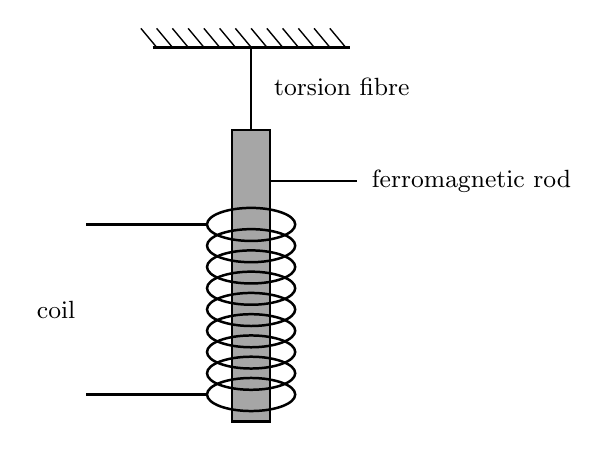
\begin{tikzpicture}[line width=0.9pt]
% 固定天花板（阴影线）
\draw (-1.25,0) -- (1.25,0);
\foreach \x in {-1.2,-1.0,...,1.2}
  \draw[line width=0.5pt] (\x,0) -- (\x-0.2,0.24);
% 扭丝
\draw (0,0) -- (0,-1.05);
\node[anchor=west,font=\small] at (0.16,-0.5) {torsion fibre};
% 铁磁棒
\draw[fill=black!35] (-0.24,-1.05) rectangle (0.24,-4.75);
% 标注：铁磁棒
\draw[line width=0.5pt] (0.24,-1.7) -- (1.35,-1.7);
\node[anchor=west,font=\small] at (1.4,-1.7) {ferromagnetic rod};
% 线圈（绕组椭圆）
\foreach \y in {-2.25,-2.52,-2.79,-3.06,-3.33,-3.60,-3.87,-4.14,-4.41}
  \draw (0,\y) ellipse (0.56 and 0.21);
% 引线
\draw (-0.56,-2.25) -- (-2.1,-2.25);
\draw (-0.56,-4.41) -- (-2.1,-4.41);
\node[anchor=east,font=\small] at (-2.1,-3.33) {coil};
\end{tikzpicture}
\end{document}
